%% Document template source: LaTeX2e template for FEUP's Project FE-UP
%% Document template author: jlopes@fe.up.pt
%% Template adapted

%% A alterar: <--ALTERAR-->

\documentclass[11pt,a4paper]{report}

%% Macros ----------------------------------------------------------------------{{{1
\newcommand{\school}{Instituto Superior de Engenharia de Lisboa}
\newcommand{\degree}{Licenciatura em Engenharia Eletrotécnica, Telecomunicações e Computadores}
\newcommand{\projisel}{Projeto ISEL 2023/24 --- LEETC}
\newcommand{\projtitle}{RCp}
\newcommand{\projsubtitle}{Subtítulo do Trabalho}
\newcommand{\projteam}{Grupo LP-07}

%% Package ---------------------------------------------------------------------{{{1
\usepackage{graphicx}           % 
\usepackage[portuguese]{babel}  % [portuges]??
\usepackage{multicol}           % 
\usepackage{longtable}          % Tables continue in the next page
\usepackage{listings}           % Programming syntax

%importados e verificar
\usepackage[utf8]{inputenc}     % accents
\usepackage{color}
\usepackage[a4paper,left=25mm,right=25mm,top=25mm,bottom=25mm,headheight=6mm,footskip=12mm]{geometry}   % Document dimensions
\usepackage{lastpage}           % 
\usepackage{fancyhdr}           % Headers and footers
\usepackage{hyperref}           % Hyper references
\usepackage{chicago}            % Bibliography style


%verificar
\usepackage[T1]{fontenc}          % PS fonts
\usepackage{newtxtext,newtxmath}  % do not use CM fonts
\usepackage{amsmath}              % multi-line and other mathematical statements
\usepackage{setspace}             % setting the spacing between lines
\usepackage[normalem]{ulem}       % various types of underlining
\usepackage{caption}              % rotating captions, sideways captions, etc.
\usepackage{float}                % tables and figures in the multi-column environment 
\usepackage{subcaption}           % for subfigures and the like
\usepackage{multirow}             % tabular cells spanning multiple rows
\usepackage[table]{xcolor}        % driver-independent color extensions
\usepackage{lipsum}               % loren dummy text
\setlength{\marginparwidth}{2cm}  % todonotes' requirements
\usepackage{todonotes}            % todo's

%% my other macros, if needed
\newcommand{\windspt}{\textsf{WindsPT\/}}
\newcommand{\windscannerpt}{\emph{Windscanner.PT\/}}
\newcommand{\class}[1]{{\normalfont\slshape #1\/}}
\newcommand{\svg}{\class{SVG}}

%% my environments for infos
\newenvironment{info}[1]{\vspace*{6mm}\color{blue}[ \begin{em} #1}
                        {\vspace*{6mm}\end{em} ]}
\newenvironment{infoopt}[1]{\vspace*{6mm}\color{blue}[ \textbf{Elemento opcional.} \begin{em} #1}
                        {\vspace*{6mm}\end{em} ]}


%% Package settings ------------------------------------------------------------{{{1
\graphicspath{{./images/}}                          % {graphicx} - Images path
\selectlanguage{portuguese}                         % {babel} - Language portuguese
\setlength{\columnsep}{3cm}                         % {multicol} - Column spacement
\definecolor{engineering}{rgb}{0.549,0.176,0.098}   % {color}
\definecolor{cloudwhite}{cmyk}{0,0,0,0.025}         % {color}
\setlength{\parindent}{0em}                         % {geometry}
\setlength{\parskip}{1ex}                           % {geometry}
\lstdefinestyle{pythoncode}                         % {listings} - Python syntax
{
    keepspaces=true,
    numbersep=5pt,

    basicstyle=\footnotesize\ttfamily,
    keywordstyle=\bfseries,
    numbers=left,                                   % where to put the line-numbers
    numberstyle=\scriptsize\texttt,                 % the size of the fonts that are used for the line-numbers
    stepnumber=1,                                   % the step between two line-numbers. If it's 1 each line will be numbered
    numbersep=8pt,                                  % how far the line-numbers are from the code
    frame=tb,
    float=htb,
    aboveskip=8mm,
    belowskip=4mm,
    backgroundcolor=\color{cloudwhite},             
    showspaces=false,                               % show spaces adding particular underscores
    showstringspaces=false,                         % underline spaces within strings
    showtabs=false,                                 % show tabs within strings adding particular underscores
    tabsize=2,                                      % sets default tabsize to 2 spaces
    captionpos=b,                                   % sets the caption-position to bottom
    breaklines=true,                                % sets automatic line breaking
    breakatwhitespace=false,                        % sets if automatic breaks should only happen at whitespace
    escapeinside={\%*}{*)},                         % if you want to add a comment within your code
    morekeywords={*,var,template,new}               % if you want to add more keywords to the set
}
\fancyhf{}                                          % {fancyhdr} clear off all default fancyhdr headers and footers
\lfoot{\small{\emph{\projtitle, \projsubtitle}}}    % {fancyhdr}
\rfoot{\small{\thepage\ / \pageref{LastPage}}}      % {fancyhdr}
\pagestyle{fancy}                                   % {fancyhdr} apply the fancy header style
\renewcommand{\headrulewidth}{0.0pt}                % {fancyhdr} no head rule
\renewcommand{\footrulewidth}{0.4pt}                % {fancyhdr}
\hypersetup{                                        % {hyperref}
    plainpages=false,
    pdfpagelayout=SinglePage,
    bookmarksopen=false,
    bookmarksnumbered=true,
    breaklinks=true,
    linktocpage,
    colorlinks=true,
    linkcolor=engineering,
    urlcolor=engineering,
    filecolor=engineering,
    citecolor=engineering,
    allcolors=engineering
}

%\usepackage{comment}               % Permite criar um segmento de comentários (/begin{comment} [...] /end{comment})
%\usepackage{xcolor}                % Colorir texto (esta versão é mais flexível do que a {color})
%\usepackage{subcaption}            % Subcaptions para figuras
%\usepackage{fullpage}              % Utilizar página inteira

%% Document start --------------------------------------------------------------{{{1
\begin{document}
\pagenumbering{roman}\setcounter{page}{1}

%% Cover -----------------------------------------------------------------------{{{1
\begin{titlepage}
    \center

    \vspace*{-12mm}
    {\large \textbf{\textsc{\school}}}\\

    \vfill

    \includegraphics[width=62mm]{<--ALTERAR-->}
    
    \vfill
    
    {\huge \textbf{\projtitle}}\\[6mm]
    {\Large \textbf{\projsubtitle}}\\
    
    \vfill
    
    \includegraphics[width=52mm]{<--ALTERAR-->}
    
    \vfill
    
    {\Large \textbf{\projisel}}\\[12mm]
    
    {\Large \textbf{Coordenação}}\\[4mm]
    {\large Geral:  \hspace*{18mm}
            De curso: }\\[6mm]
    
    {\Large \textbf{\projteam}}\\[4mm]
    {\large Supervisor: \hspace*{12mm}
            Monitor: }\\[6mm]
    
    {\Large \textbf{Estudante}}\\[4mm]
    {\large Nuno Brito $<$A46948@alunos.isel.pt$>$ \hspace*{12mm}
    
    \renewcommand{\today}{<--ALTERAR-->}
    \today
    
\end{titlepage}

%% TOC -------------------------------------------------------------------------{{{1
\tableofcontents

%% List of figures -------------------------------------------------------------{{{1
\listoffigures
\addcontentsline{toc}{chapter}{Lista de figuras}


%% List of tables --------------------------------------------------------------{{{1
\listoftables
\addcontentsline{toc}{chapter}{Lista de tabelas}

%% Acronyms --------------------------------------------------------------------{{{1
\chapter*{Lista de acrónimos}
\addcontentsline{toc}{chapter}{Lista de acrónimos}

\begin{flushleft}
\begin{tabular}{l p{0.8\linewidth}}
ADT      & Abstract Data Type\\
API      & Application Programming Interface\\
WWW      & World Wide Web
\end{tabular}
\end{flushleft}

%% Glossary --------------------------------------------------------------------{{{1
\chapter*{Glossário}
\addcontentsline{toc}{chapter}{Glossário}

\begin{description}
    \item[Operating system] \hfill \\
        Text
    \item[Browser] \hfill \\
        Text
    \item[Package monitor] \hfill \\
        Text
    \item[Windows] \hfill \\
        Text
    \item[Rolling distribuition] \hfill \\
        Text
    \item[openSUSE Tumbleweed] \hfill \\
        Text
    \item[Wireshark] \hfill \\
        Text
    \item[LibreWolf] \hfill \\
        Text
    \item[XAMPP] \hfill \\
        Text
    \item[HTTP] \hfill \\
        Text
    \item[TCP] \hfill \\
        Text
    \item[Apache2] \hfill \\
        Text
    \item[Localhost] \hfill \\
        Text
    \item[Socket] \hfill \\
        Text
    \item[Python] \hfill \\
        Text
    \item[TLS] \hfill \\
        Text
    \item[Firewall] \hfill \\
        Text
    \item[VPN] \hfill \\
        Text
    \item[SSL] \hfill \\
        Text
    \item[] \hfill \\
        Text
    \item[] \hfill \\
        Text
    \item[] \hfill \\
        Text
    \item[] \hfill \\
        Text
    \item[] \hfill \\
        Text
    \item[] \hfill \\
        Text
    \item[] \hfill \\
        Text

\item[bash] \hfill \\
  Bash é uma \emph{shell Unix} e uma linguagem de comando escrita
  em 1989 por Brian Fox para o Projeto GNU como um substituto de
  software livre para a \emph{Bourne shell}.
\item[firewall] \hfill \\
  Em computação, uma \emph{firewall} é um sistema de segurança de rede
  que monitoriza e controla o tráfego de entrada e saída da rede
  com base em regras de segurança predeterminadas.
  Uma \emph{firewall} normalmente estabelece uma barreira entre uma
  rede confiável e uma rede não confiável, como a Internet.
\item[Glossário] \hfill \\
  Glossário é uma espécie de pequeno dicionário específico para
  palavras e expressões pouco conhecidas presentes num texto, seja
  por serem de natureza técnica, regional ou de outro idioma.
\end{description}

%% Chapter: introduction -------------------------------------------------------{{{1
\chapter{Introduction}
%% display headers & footers
\pagestyle{fancy}
%% main page numbers with arabic numerals
\pagenumbering{arabic}\setcounter{page}{1}



%% Chapter: project ------------------------------------------------------------{{{1
\chapter{Phase 1}
    \section{Milestones}
        \begin{itemize}
            \item Setup apache2 web server in localhost
            \item Access web server locally (http://127.0.0.1/)
            \item Access web server from a remote computer
            \item Use wireshark in a remote host to capture packages from the server
            \item Compare the HTTP headers sent by the client and the server
            \item Develop a simple barebones HTTP webclient
            \item Establish a TCP connection to the server
            \item Request the base webpage
        \end{itemize}
        
    \section{WebClient requirements}
        \begin{itemize}
            \item HTTP library forbidden
            \item Establish TCP connection using available sockets library - send/receive the HTTP request/reply
            \item Output HTTP reply to the user
            \item - Optional - act to the various HTTP replies
            \item Text-only application
        \end{itemize}

    \subsection{Software}
        \item Local server side
            \subitem Operating system: Windows 11 x64
            \subitem WebServer: XAMPP x64 8.2.12-0-VS16 for windows
        Disclaimer: the versions listed below might not be the latest, by present date, given the nature of rolling distribuitions software updates.
        \item Client side
            \subitem Operating system: openSUSE Tumbleweed
            \subitem Browser: LibreWolf version 123.0-1
            \subitem Package monitor: Wireshark version 4.2.3 (Git commit b0da86c196d1).
    
    \subsection{WebClient - Python Code}
        \lstset{style=pythoncode}
        \lstinputlisting[language=python, caption=Simple HTTP WebClient using sockets in python]{webclient/httpsocketv3.py}
        The code was adapted to be simple and cycle through the various request messages without any user input.
        Modifiable variables include serverName, serverPort and the httpTestMessages list.
    
    \subsection{List of headers and replies}
            \textbf{Request:} GET /dashboard/ HTTP/1.1\r\nHost:127.24.1.12\r\n\r\n
            \textbf{Reply:} HTTP/1.1 200 OK
                Meaning: this header complies with what the server expects from a webclient request.
            \textbf{Request:} GET /dashboard HTTP/1.1\r\nHost:127.24.1.12\r\n\r\n
            \textbf{Reply:} HTTP/1.1 301 Moved Permanently
                Meaning: this header request a relative directory without a forward slash at the end, prompting the server to reply with a "moved" answer.
            \textbf{Request:} PUT / HTTP/1.1\r\nHost:127.24.1.12\r\n\r\n
            \textbf{Reply:} HTTP/1.1 302 Found
                Meaning: this header request is an upload request to an unexistent directory.
            \textbf{Request:} GET /dashboard HTTP/1.\r\nHost:127.24.1.12\r\n\r\n
            \textbf{Reply:} HTTP/1.1 400 Bad Request
                Meaning: this header request, although it has an invalid directory, has the HTTP protocol version badly writen (HTTP/1.1 vs. actual HTTP/1.) which causes
                a "bad request" reply from the server.
            \textbf{Request:} GET /dashboard/index.htm HTTP/1.1\r\nHost:127.24.1.12\r\n\r\n
            \textbf{Reply:} HTTP/1.1 404 Not Found
                Meaning: this header request tries to get a file that doesn't exist in the local server.
            \textbf{Request:} PUT /d HTTP/1.1\r\nHost:127.24.1.12\r\n\r\n
            \textbf{Reply:} HTTP/1.1 405 Method Not Allowed
                Meaning: this header request tries to upload something to the relative directory "d".
        
    \subsection{Software install steps}
        Step-by-step instructions performed
        Xampp install
        wireshark install
        wireshark settings
        wireshark filters

        Webclient output
        Wireshark outputs browser
        Wireshark outputs webclient

        % Yo reduce the ammount of pictures! Or maybe side by side 
        \begin{tabular}{ l r }
            text & \includegraphics[scale=1.0]{install_xampp01} \\ % 0.3 scale!
            text & \includegraphics[scale=1.0]{install_xampp02} \\
            text & \includegraphics[scale=1.0]{install_xampp03} \\
            text & \includegraphics[scale=1.0]{install_xampp04} \\
            text & \includegraphics[scale=1.0]{install_xampp05} \\
            text & \includegraphics[scale=1.0]{install_xampp06} \\
            text & \includegraphics[scale=1.0]{install_xampp07} \\
            text & 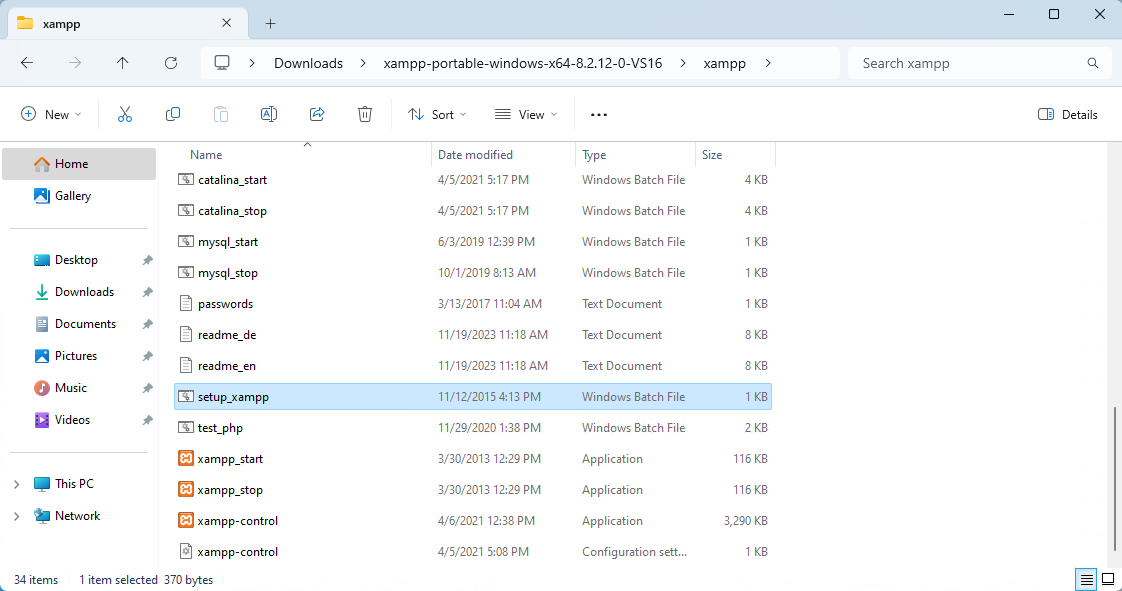
\includegraphics[scale=1.0]{install_xampp08} \\
            text & 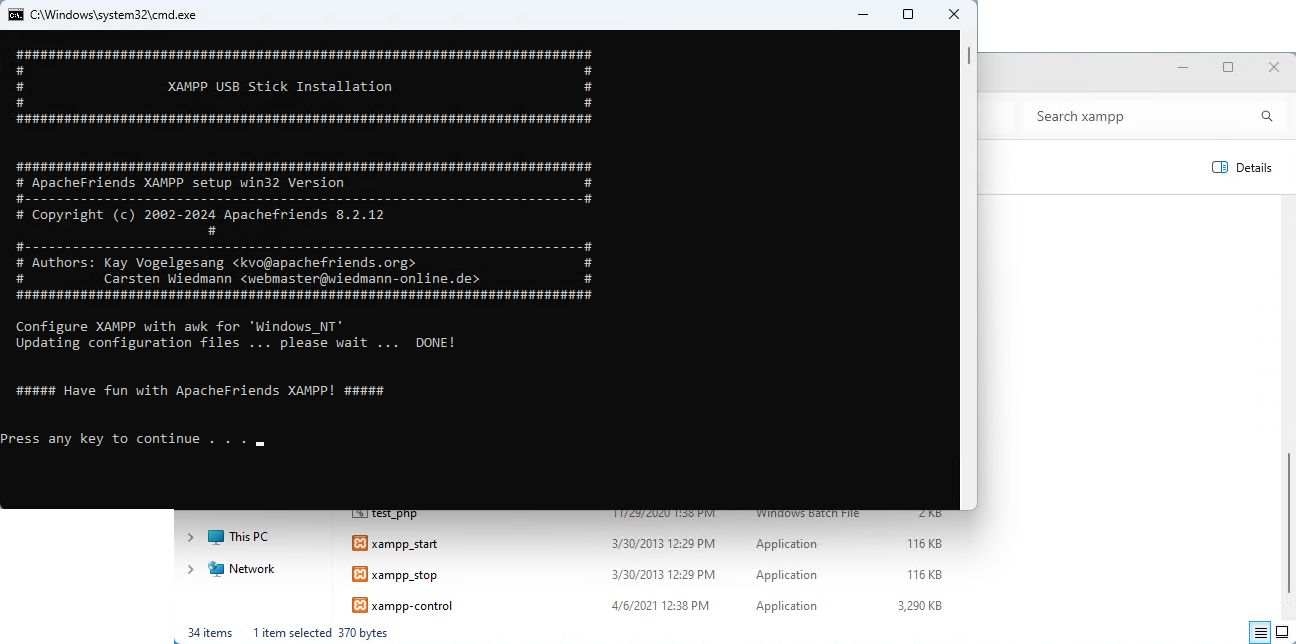
\includegraphics[scale=1.0]{install_xampp09} \\
            text & 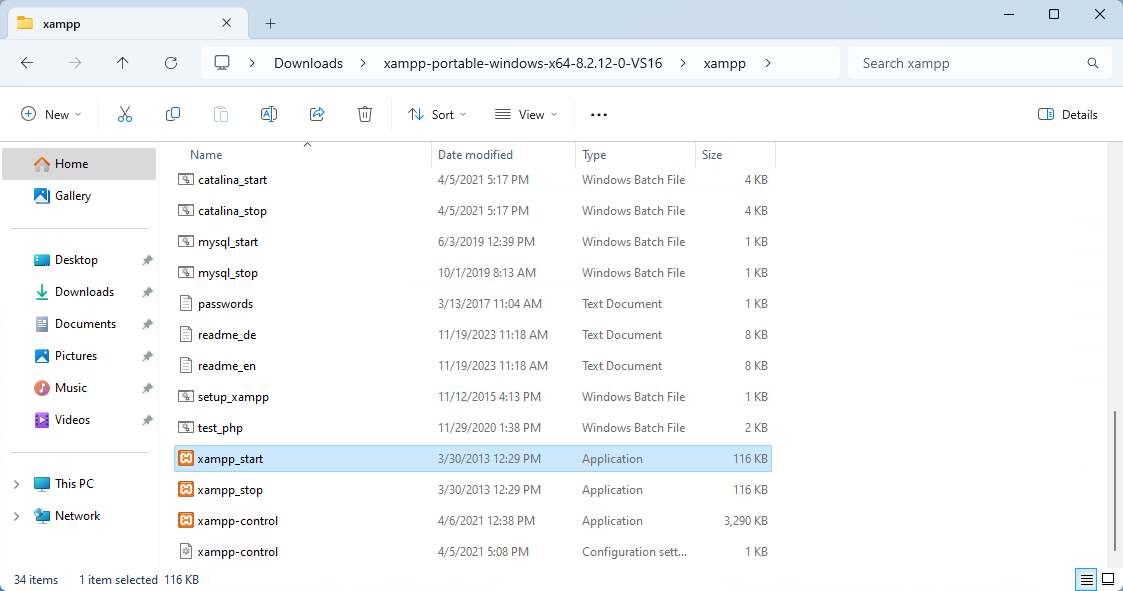
\includegraphics[scale=1.0]{install_xampp10} \\
            text & \includegraphics[scale=1.0]{install_xampp11} \\
            text & \includegraphics[scale=1.0]{install_xampp12} \\
            text & 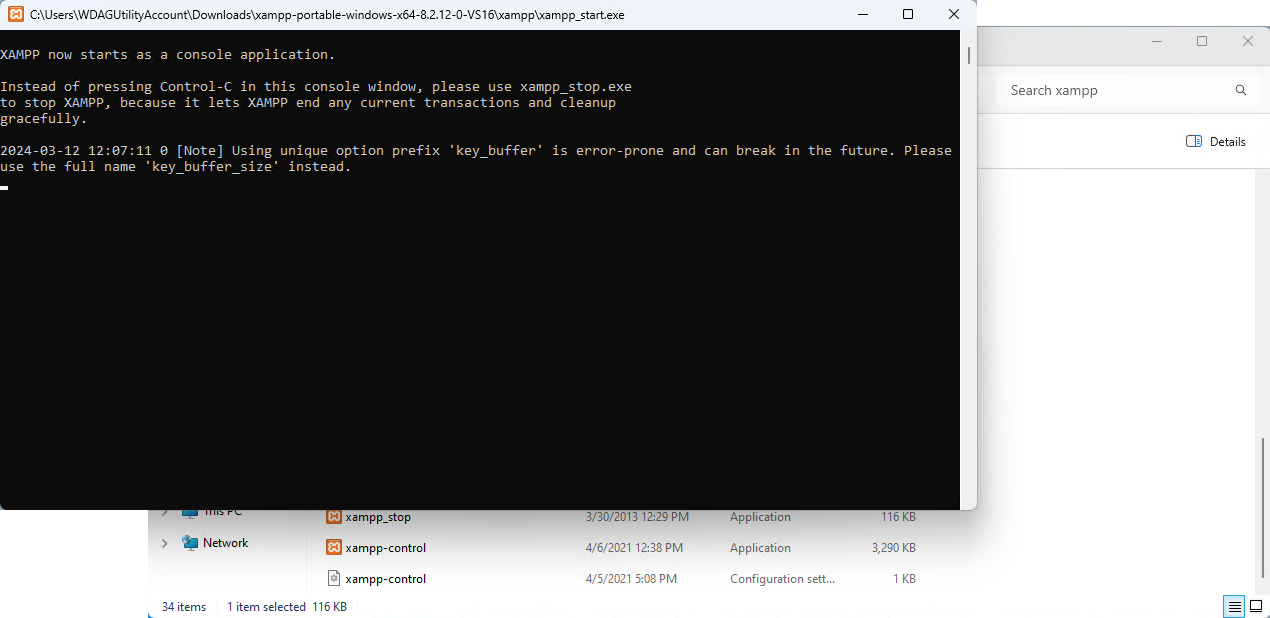
\includegraphics[scale=1.0]{install_xampp13} \\
            text & 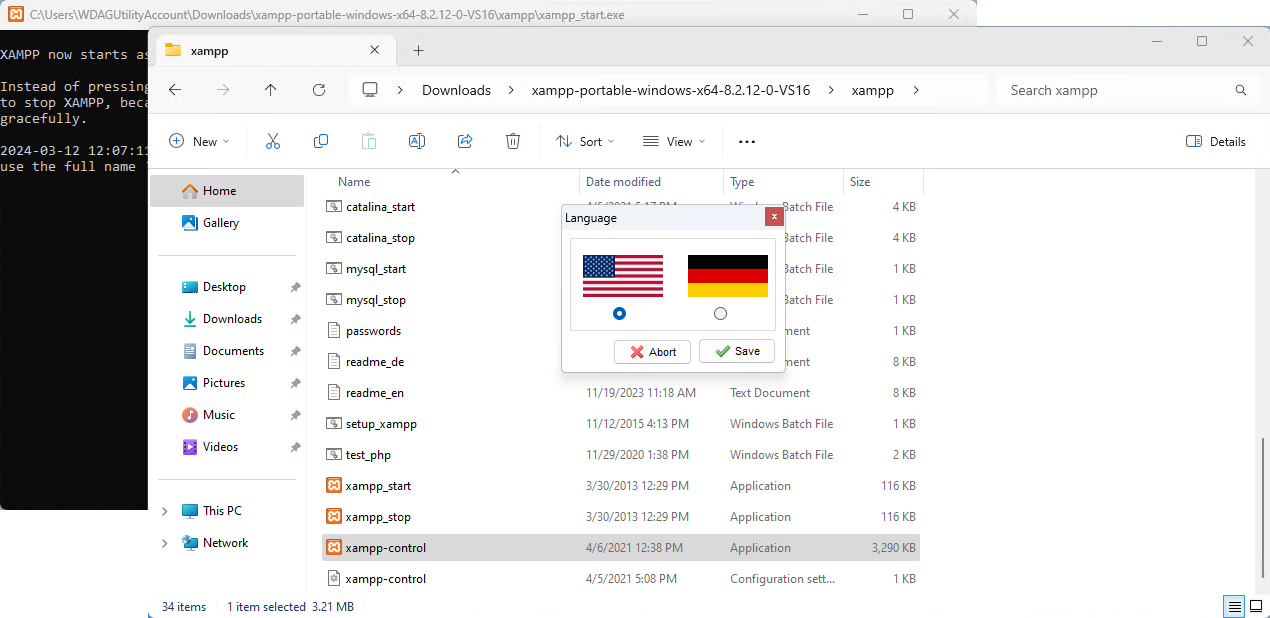
\includegraphics[scale=1.0]{install_xampp14} \\
            text & 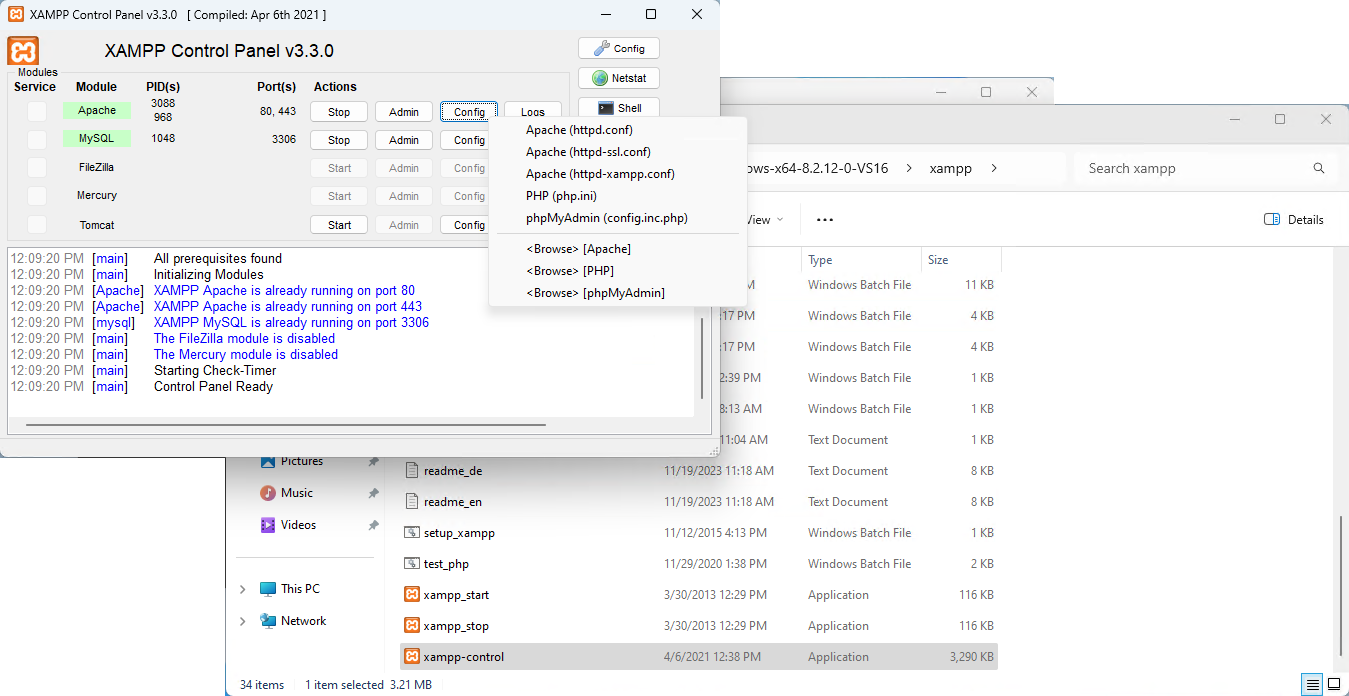
\includegraphics[scale=1.0]{install_xampp15} \\
            text & 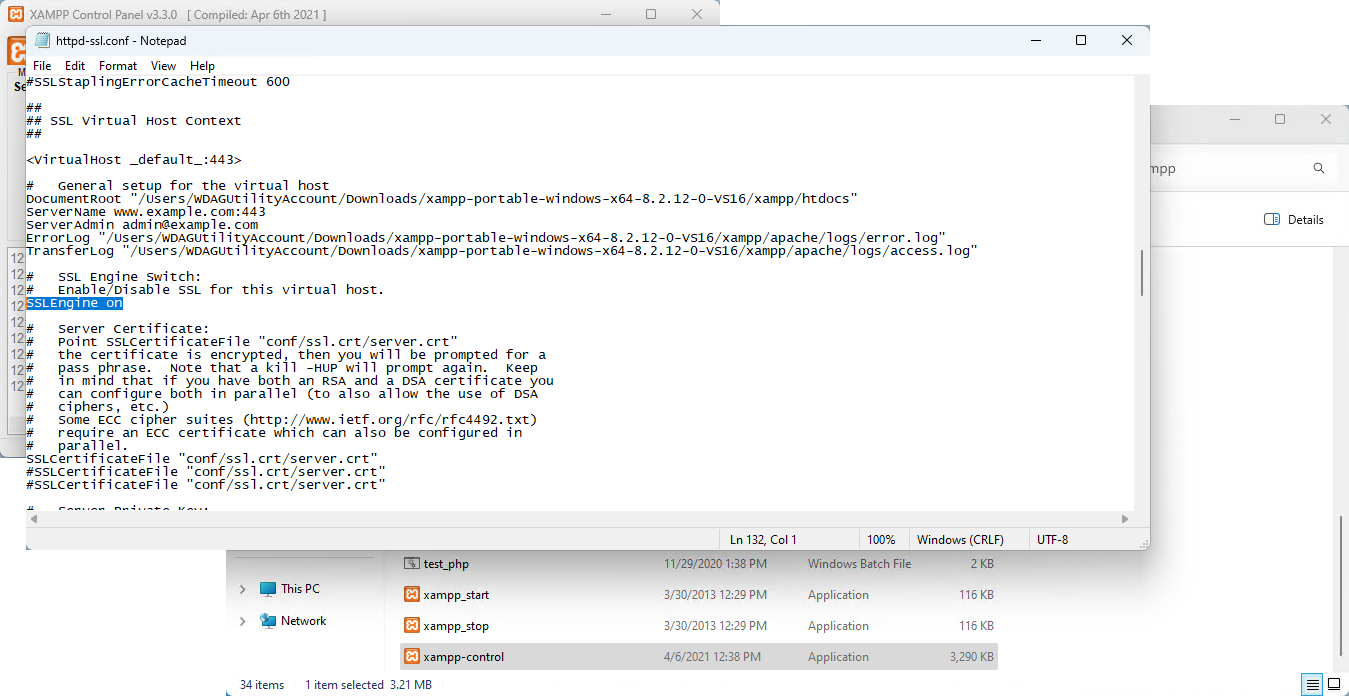
\includegraphics[scale=1.0]{install_xampp16} \\
            text & 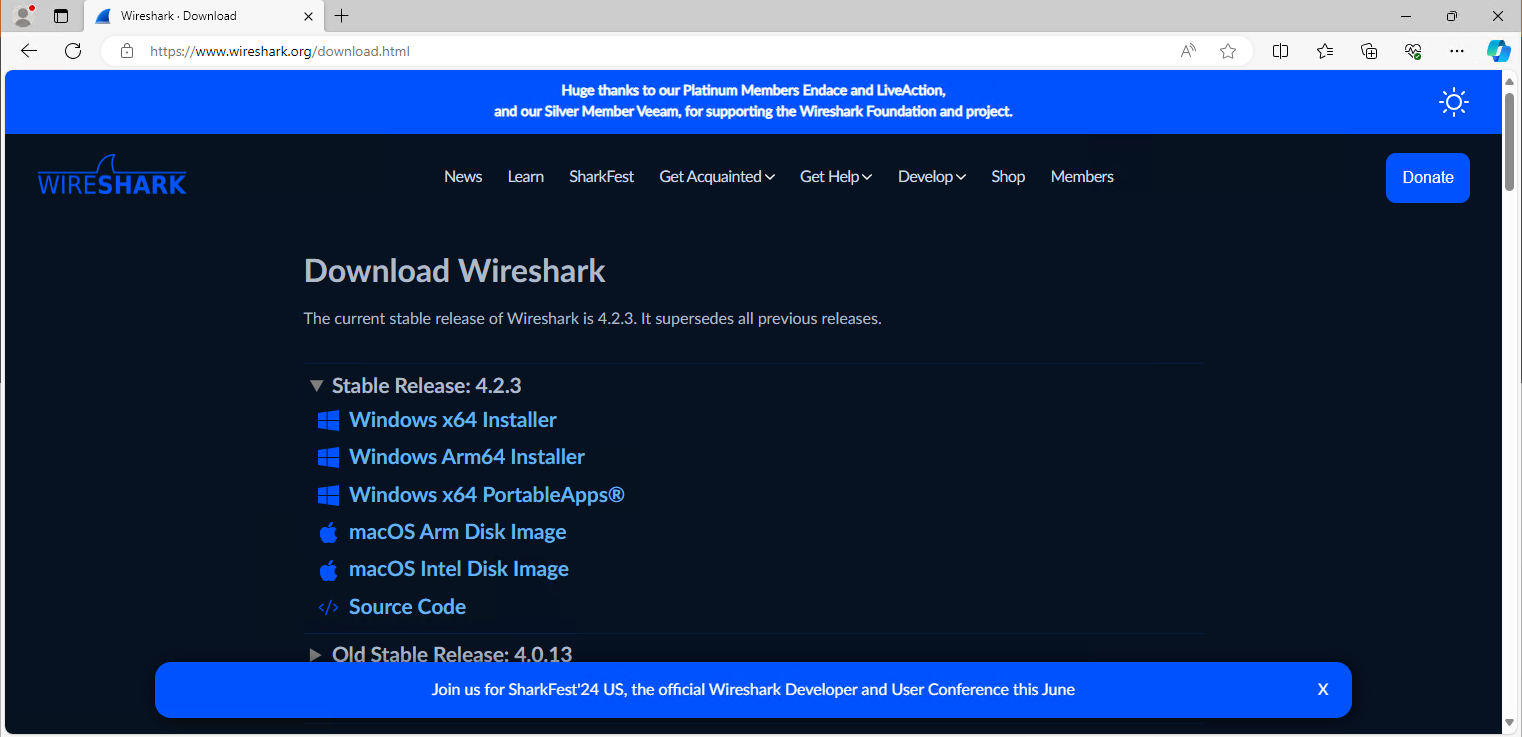
\includegraphics[scale=1.0]{install_wireshark01} \\
            text & 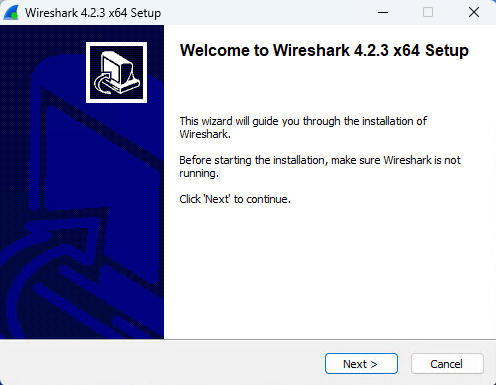
\includegraphics[scale=1.0]{install_wireshark02} \\
            text & 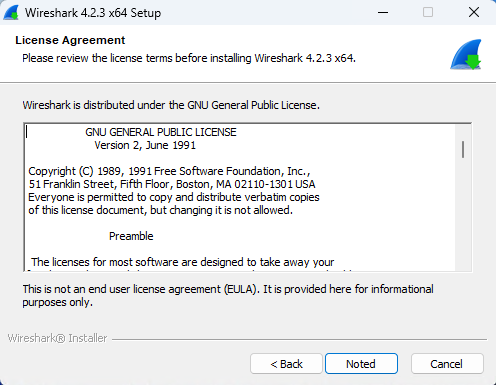
\includegraphics[scale=1.0]{install_wireshark03} \\
            text & 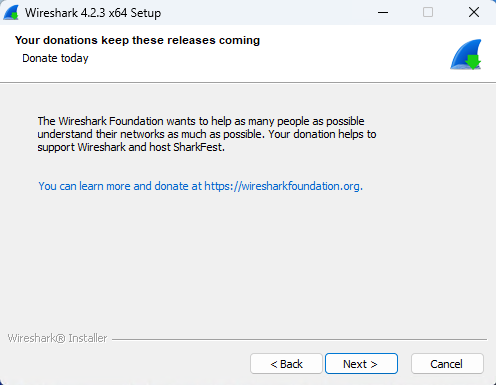
\includegraphics[scale=1.0]{install_wireshark04} \\
            text & 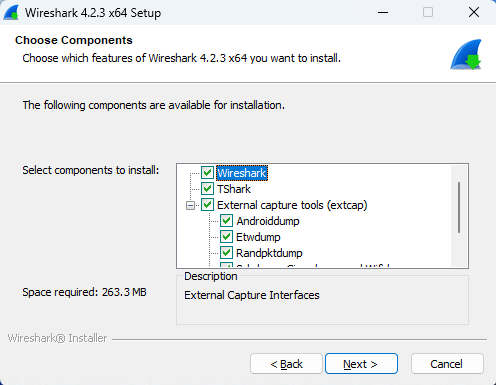
\includegraphics[scale=1.0]{install_wireshark05} \\
            text & 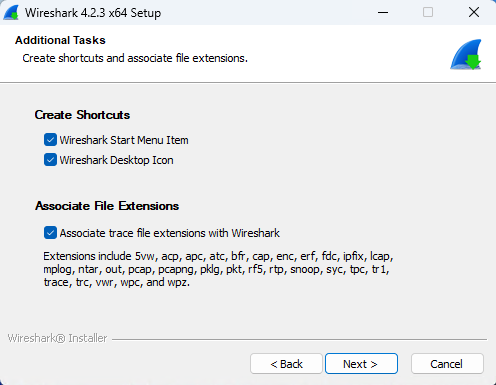
\includegraphics[scale=1.0]{install_wireshark06} \\
            text & 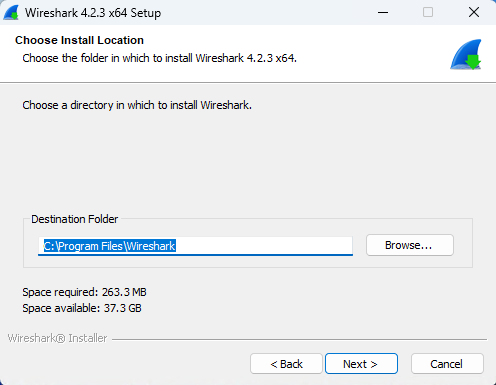
\includegraphics[scale=1.0]{install_wireshark07} \\
            text & 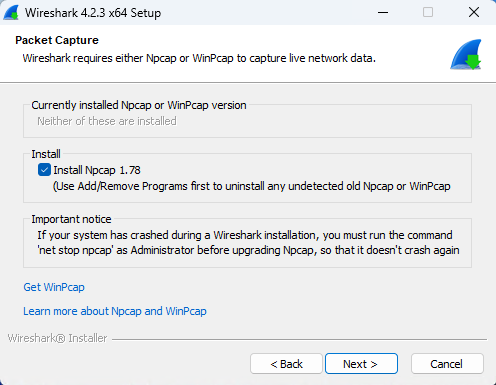
\includegraphics[scale=1.0]{install_wireshark08} \\
            text & 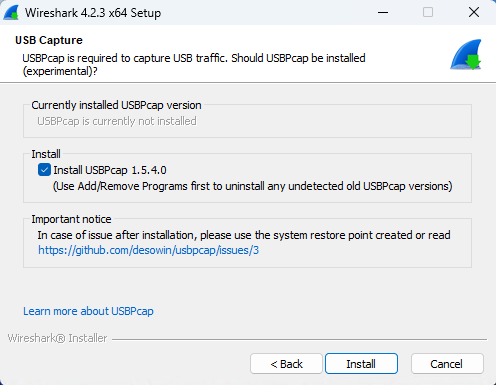
\includegraphics[scale=1.0]{install_wireshark09} \\
            text & 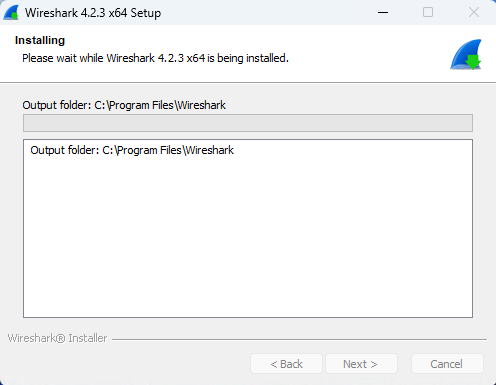
\includegraphics[scale=1.0]{install_wireshark10} \\
            text & 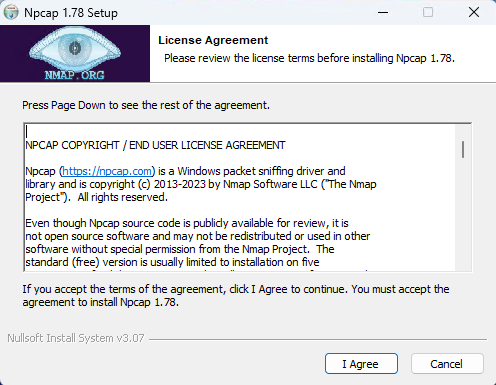
\includegraphics[scale=1.0]{install_wireshark11} \\
            text & 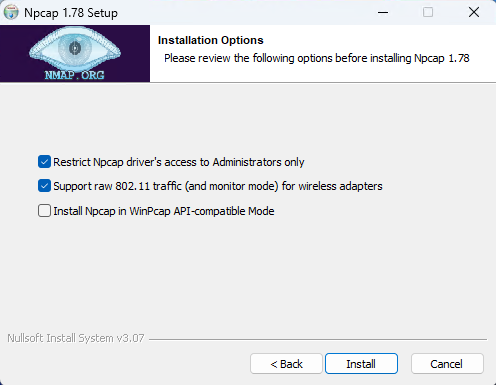
\includegraphics[scale=1.0]{install_wireshark12} \\
            text & 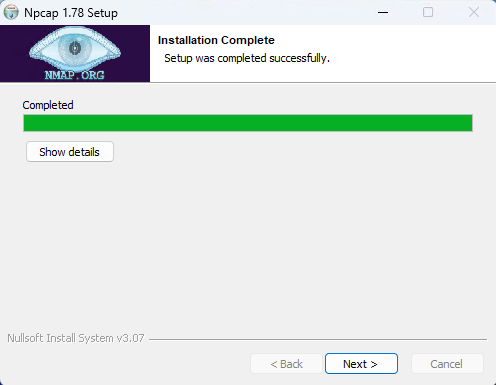
\includegraphics[scale=1.0]{install_wireshark13} \\
            text & 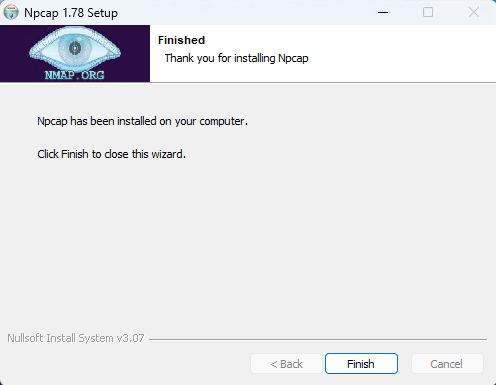
\includegraphics[scale=1.0]{install_wireshark14} \\
            text & 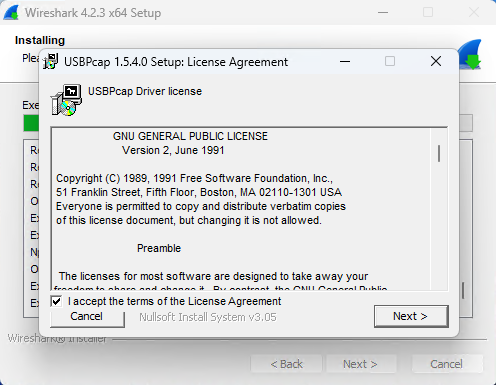
\includegraphics[scale=1.0]{install_wireshark15} \\
            text & 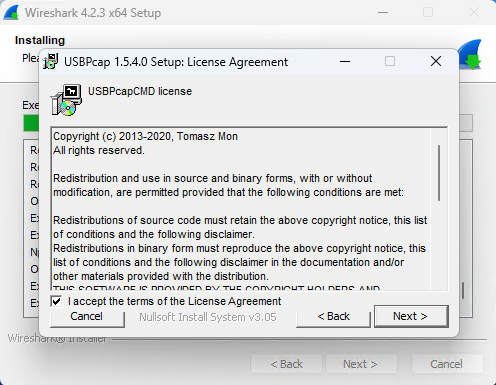
\includegraphics[scale=1.0]{install_wireshark16} \\
            text & 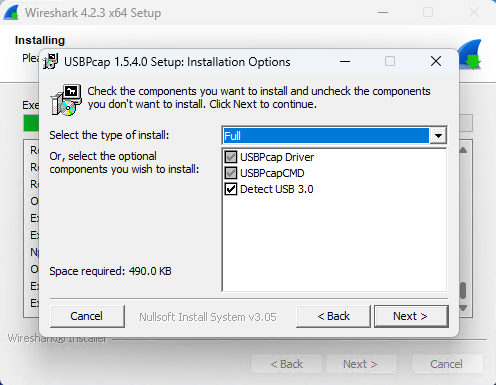
\includegraphics[scale=1.0]{install_wireshark17} \\
            text & 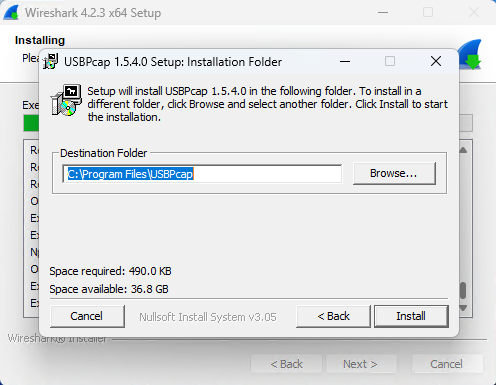
\includegraphics[scale=1.0]{install_wireshark18} \\
            text & 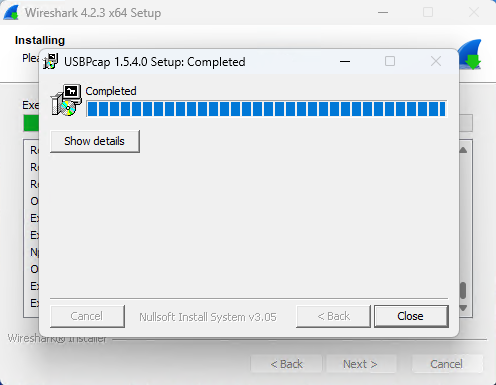
\includegraphics[scale=1.0]{install_wireshark19} \\
            text & 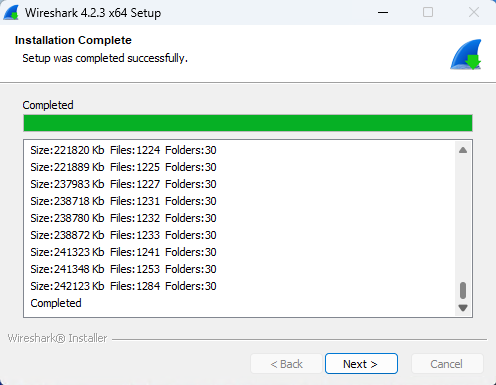
\includegraphics[scale=1.0]{install_wireshark20} \\
            text & 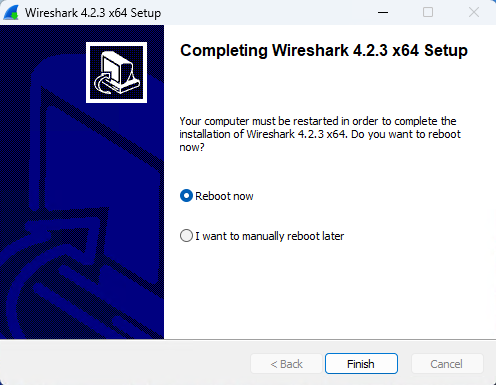
\includegraphics[scale=1.0]{install_wireshark21} \\
        \end{tabular}

    \subsection{Configurations}
        LibreWolf using deprecated TLS and unsecured sites enabled
        SSLEngine disabled in apache2 to ease access with http protocol
        %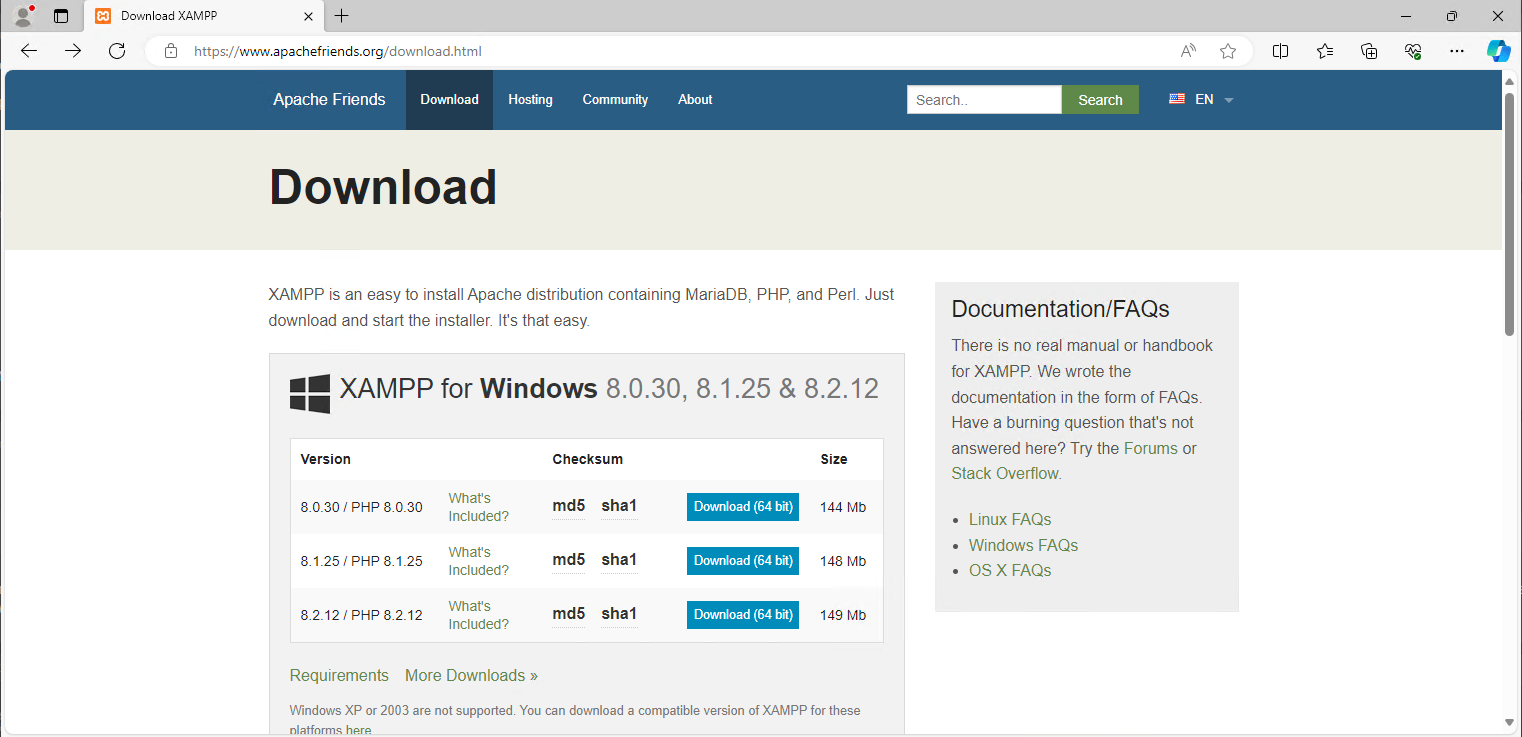
\includegraphics[scale=1.0]{xampp01} \\
        %<=++figure sslengine off++=>
        %<=++figure access from localhost++=>
        %<=++figure access from 127.0.0.1++=>
        %<=++figure access from anotherhost++=>
        %<=++figure wireshark capture from another host++=>
        
        \begin{multicols}{2}
        [Install]
        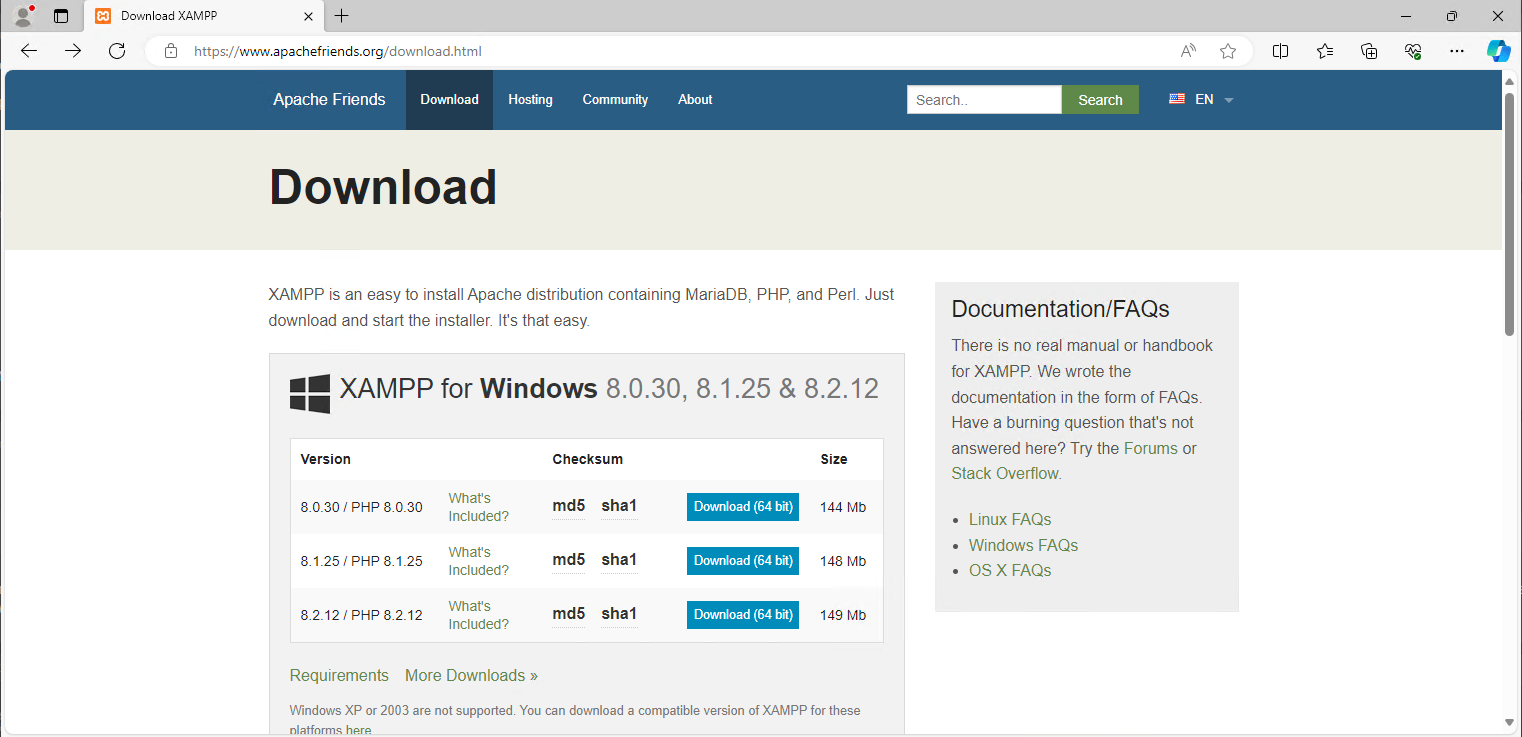
\includegraphics[scale=1.0]{1}

%% Chapter: recomendations -----------------------------------------------------{{{1
\section{Problems and resolutions}
    Python code: default system came with python2. Python3 installed.
    Encrypted html body: since the xampp server is running in a laptop at home and to make some progress i have to work remotely via vpn, the content came encrypted.
    Default http protocol SSL: disabled in apache2 the ssl engine

%% Chapter: conclusions --------------------------------------------------------{{{1

%% Bibliography ----------------------------------------------------------------{{{1
\renewcommand{\bibname}{Referências bibliográficas}
\bibliographystyle{chicago}
\bibliography{refs}
\addcontentsline{toc}{chapter}{\refname}  % add it to table of contents

%% Appendix --------------------------------------------------------------------{{{1
\appendix
\chapter{Um Apêndice}
%%1}}}

\end{document}
